\documentclass{article}
\usepackage[utf8]{inputenc}
\usepackage{graphicx}
\graphicspath{ {images/} }
\usepackage{mathtools}
\usepackage{amssymb}



\title{ECE521A1 Report}
\author{Wenjia Liu - 1000522589\\Jiashen Wang - 1001259568\\Seunghyun Cho - 1001681325}



\begin{document}

\maketitle

\section{Euclidean distance function}
Include the snippets of the Python code.

\begin{verbatim}
def euclidianDist(a, b):
    x_z = (tf.expand_dims(a,0) - tf.expand_dims(b,1))
    return tf.transpose(tf.reduce_sum(tf.multiply(x_z, x_z), 2))
  
\end{verbatim}


\section{Making Predictions for Regression}
\subsection{Choosing the nearest neighbours}
Include the relevant snippets of your Python code.
\begin{verbatim}
def pickKNearestNeighboursUnscaled(DistMatrix, k):
    length = tf.shape(DistMatrix)[1]
    
    values, indices = tf.nn.top_k(-DistMatrix, k)
    range = tf.range(length)
    
    rangeblock = tf.expand_dims(tf.expand_dims(range, 0),0)
    indexblock = tf.expand_dims(indices, 2)
    
    truth_matrix = tf.reduce_sum(tf.to_float(tf.equal(rangeblock, indexblock)),1)

    return truth_matrix

def pickKNearestNeighbours(DistMatrix, k):
    length = tf.shape(DistMatrix)[1]
    
    values, indices = tf.nn.top_k(-DistMatrix, k)
    range = tf.range(length)
    
    rangeblock = tf.expand_dims(tf.expand_dims(range, 0),0)
    indexblock = tf.expand_dims(indices, 2)
    
    truth_matrix = tf.reduce_sum(tf.to_float(tf.equal(rangeblock, indexblock)),1)

    return truth_matrix / tf.to_float(k)
\end{verbatim}

\subsection{Prediction}



The best k using the validation error is k=1, which has the minimum validation MSE loss.\\
\\

\begin{center}
\centering
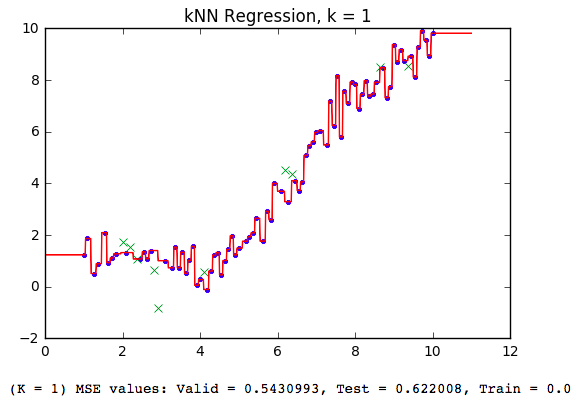
\includegraphics[scale=0.6]{1.png}

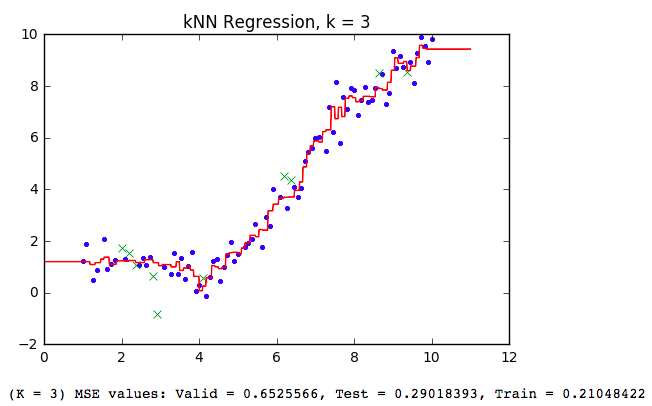
\includegraphics[scale=0.6]{2.png}

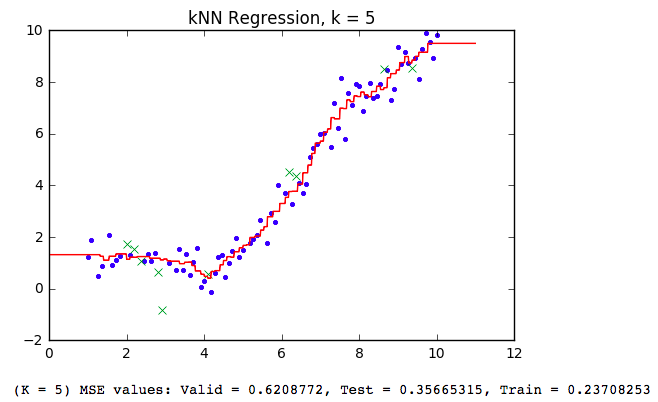
\includegraphics[scale=0.6]{3.png}

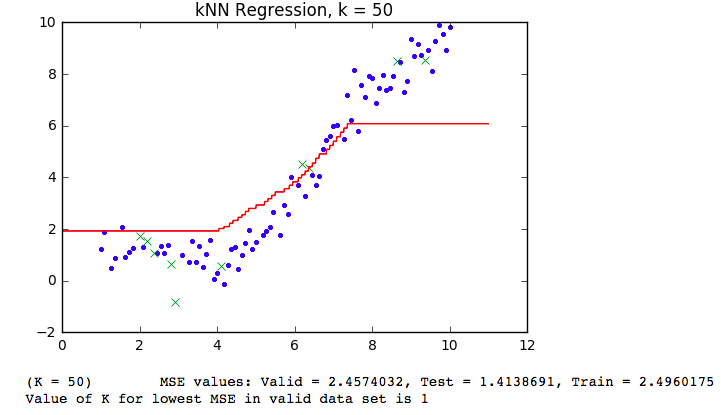
\includegraphics[scale=0.6]{4.png}
\end{center}


The plot shows that for k=1, there is an overfitting problem, so the curve has many wiggles, including much noise information. However, if k is too large, such as k=50, the difference between predicted y value and true y value is obvious. So in summary, k = 5 is the best.


\section{Making Predictions for Classification}
\subsection{Predicting class label}
Include the relevant snippet of code for this task.

\begin{verbatim}
def predictFinalValue(inputX, trainX, trainY, K):
    Knearest = pickKNearestNeighboursUnscaled(euclidianDist(inputX, trainX), K)
    predictionMatrix = tf.multiply(Knearest, trainY + 1)

    outputY = tf.zeros(0)    
    for i in range(0, runCount):
        y, idx, count = tf.unique_with_counts(predictionMatrix[i])
        count2 = tf.slice(count, [1], tf.shape(count)-1)
        item_class = tf.expand_dims(y[tf.argmax(count2)+1],0)
        outputY = tf.concat([outputY, item_class],0)
    
    outputY = outputY - 1
    return tf.to_int32(outputY)
\end{verbatim}

\subsection{Face recognition using k-NN}
For k = 1, validation accuracy is 61/92;\\
For k = 5, validation accuracy is 52/92;\\
For k = 10, validation accuracy is 51/92;\\
For k = 25, validation accuracy is 52/92;\\
For k = 50, validation accuracy is 49/92;\\
For k = 100, validation accuracy is 43/92;\\
For k = 200, validation accuracy is 28/92;\\\\
The value of k that achieves the best validation accuracy for person is 1 \\\\
For k = 1, test accuracy is 66/93;\\
For k = 5, test accuracy is 63/93;\\
For k = 10, test accuracy is 63/93;\\
For k = 25, test accuracy is 62/93;\\
For k = 50, test accuracy is 52/93;\\
For k = 100, test accuracy is 44/93;\\
For k = 200, test accuracy is 34/93;\\\\

\begin{figure}
    \caption{Example of a test point that is classified incorrect}
    \centering
        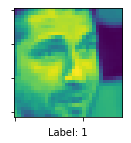
\includegraphics[scale=0.6]{5.png}
\end{figure}

\begin{figure}
    \caption{k=10 nearest neighbors that is not the same as true person}
    \centering
        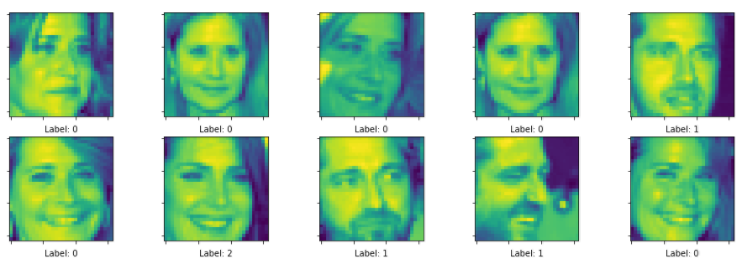
\includegraphics[scale=0.6]{6.png}
\end{figure}

\subsection{Gender recognition using k-NN}
For K = 1 validation accuracy is 84/92\\
For K = 5 validation accuracy is 84/92\\
For K = 10 validation accuracy is 80/92\\
For K = 25 validation accuracy is 83/92\\
For K = 50 validation accuracy is 82/92\\
For K = 100 validation accuracy is 78/92\\
For K = 200  validation accuracy is 71/92\\\\
The value of k that achieves the best validation accuracy for gender is 1 or 2\\\\
For K = 1 test accuracy is: 86/93\\
For K = 5  test accuracy is: 84/93\\
For K = 10  test accuracy is: 82/93\\
For K = 25  test accuracy is: 82/93\\
For K = 50  test accuracy is: 80/93\\
For K = 100  test accuracy is: 77/93\\
For K = 200  test accuracy is: 68/93\\

\begin{figure}
    \caption{Example of a test point that is classified incorrect}
    \centering
        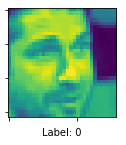
\includegraphics[scale=0.6]{7.png}
\end{figure}

\begin{figure}
    \caption{k=10 nearest neighbors that is not the same as true person}
    \centering
        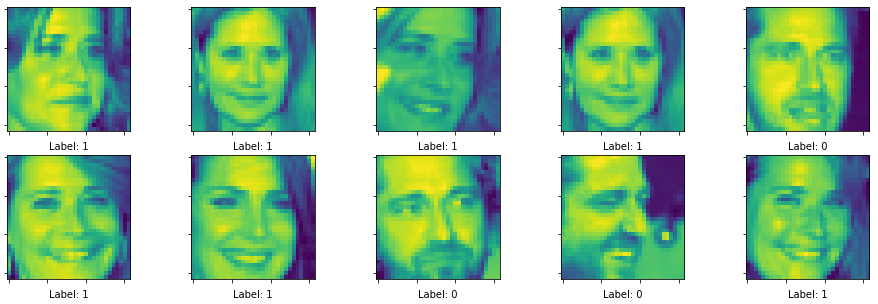
\includegraphics[scale=0.6]{8.png}
\end{figure}

\end{document}
